%\chapter{Vorlesung}
Bei $n$ Elementen sollte die Hashtabelle $m=n^2$ groß sein.\\
Für die universellen Hashfunktionen \[\mathcal{H}_{p,m} = \{ h_{a,b}(k)=(a\cdot k + b) \mod{p} \mod{m}| 0<a<p,~0\leq b < p \}\]\\
$\binom{n}{1}$ Schlüsselpaare $(k,l)$ mit $k \neq l$
\[ E(\text{\#Kollisionen}) \leq \binom{n}{2}\cdot \frac{1}{m}\footnote{Universalität von $\mathcal{H}$}=\frac{n(n-1)}{2}\cdot\frac{1}{n^2}\leq\frac{1}{2} \]
\paragraph{Idee}
Zweistufiges Verfahren:
\begin{itemize}
	\item primäre Hashfunktion für Tabelle der Größe $m=n$
\end{itemize}
\begin{figure}[H]
\centering
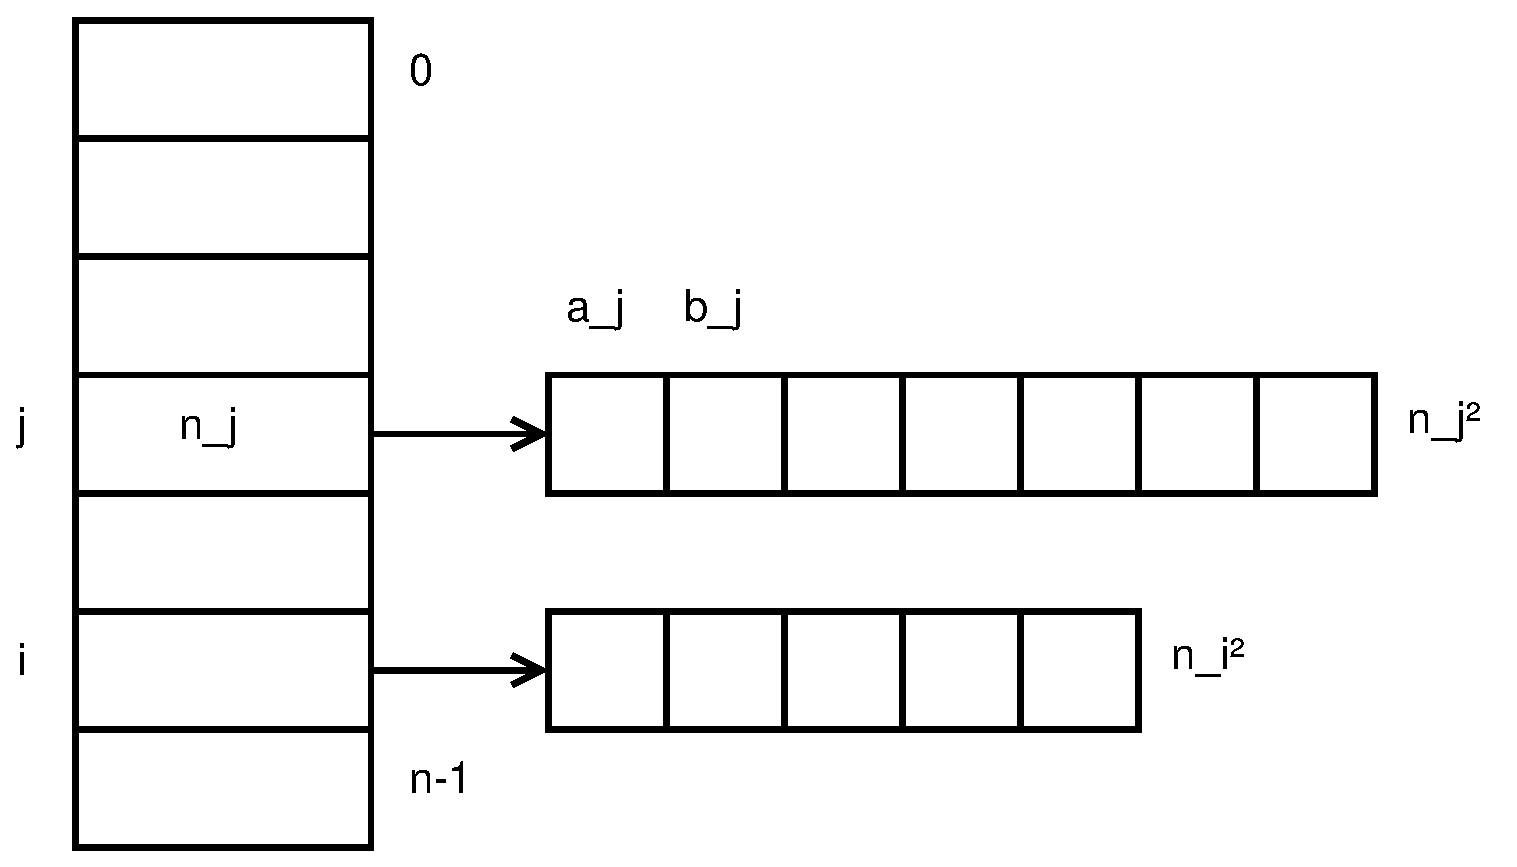
\includegraphics[width=0.5\linewidth]{15/Grafik/PHsching}
\caption[Perfektes Hashing]{Perfektes Hashing}
\label{fig:PHsching}
\end{figure}
\part{Graphen-Algorithmen}
\chapter{Einführung}
\[ G=(V,E)~~~V\text{ vertices, }E\text{ edges}~~~E\subseteq V \times V \]

\begin{figure}[H]
\centering
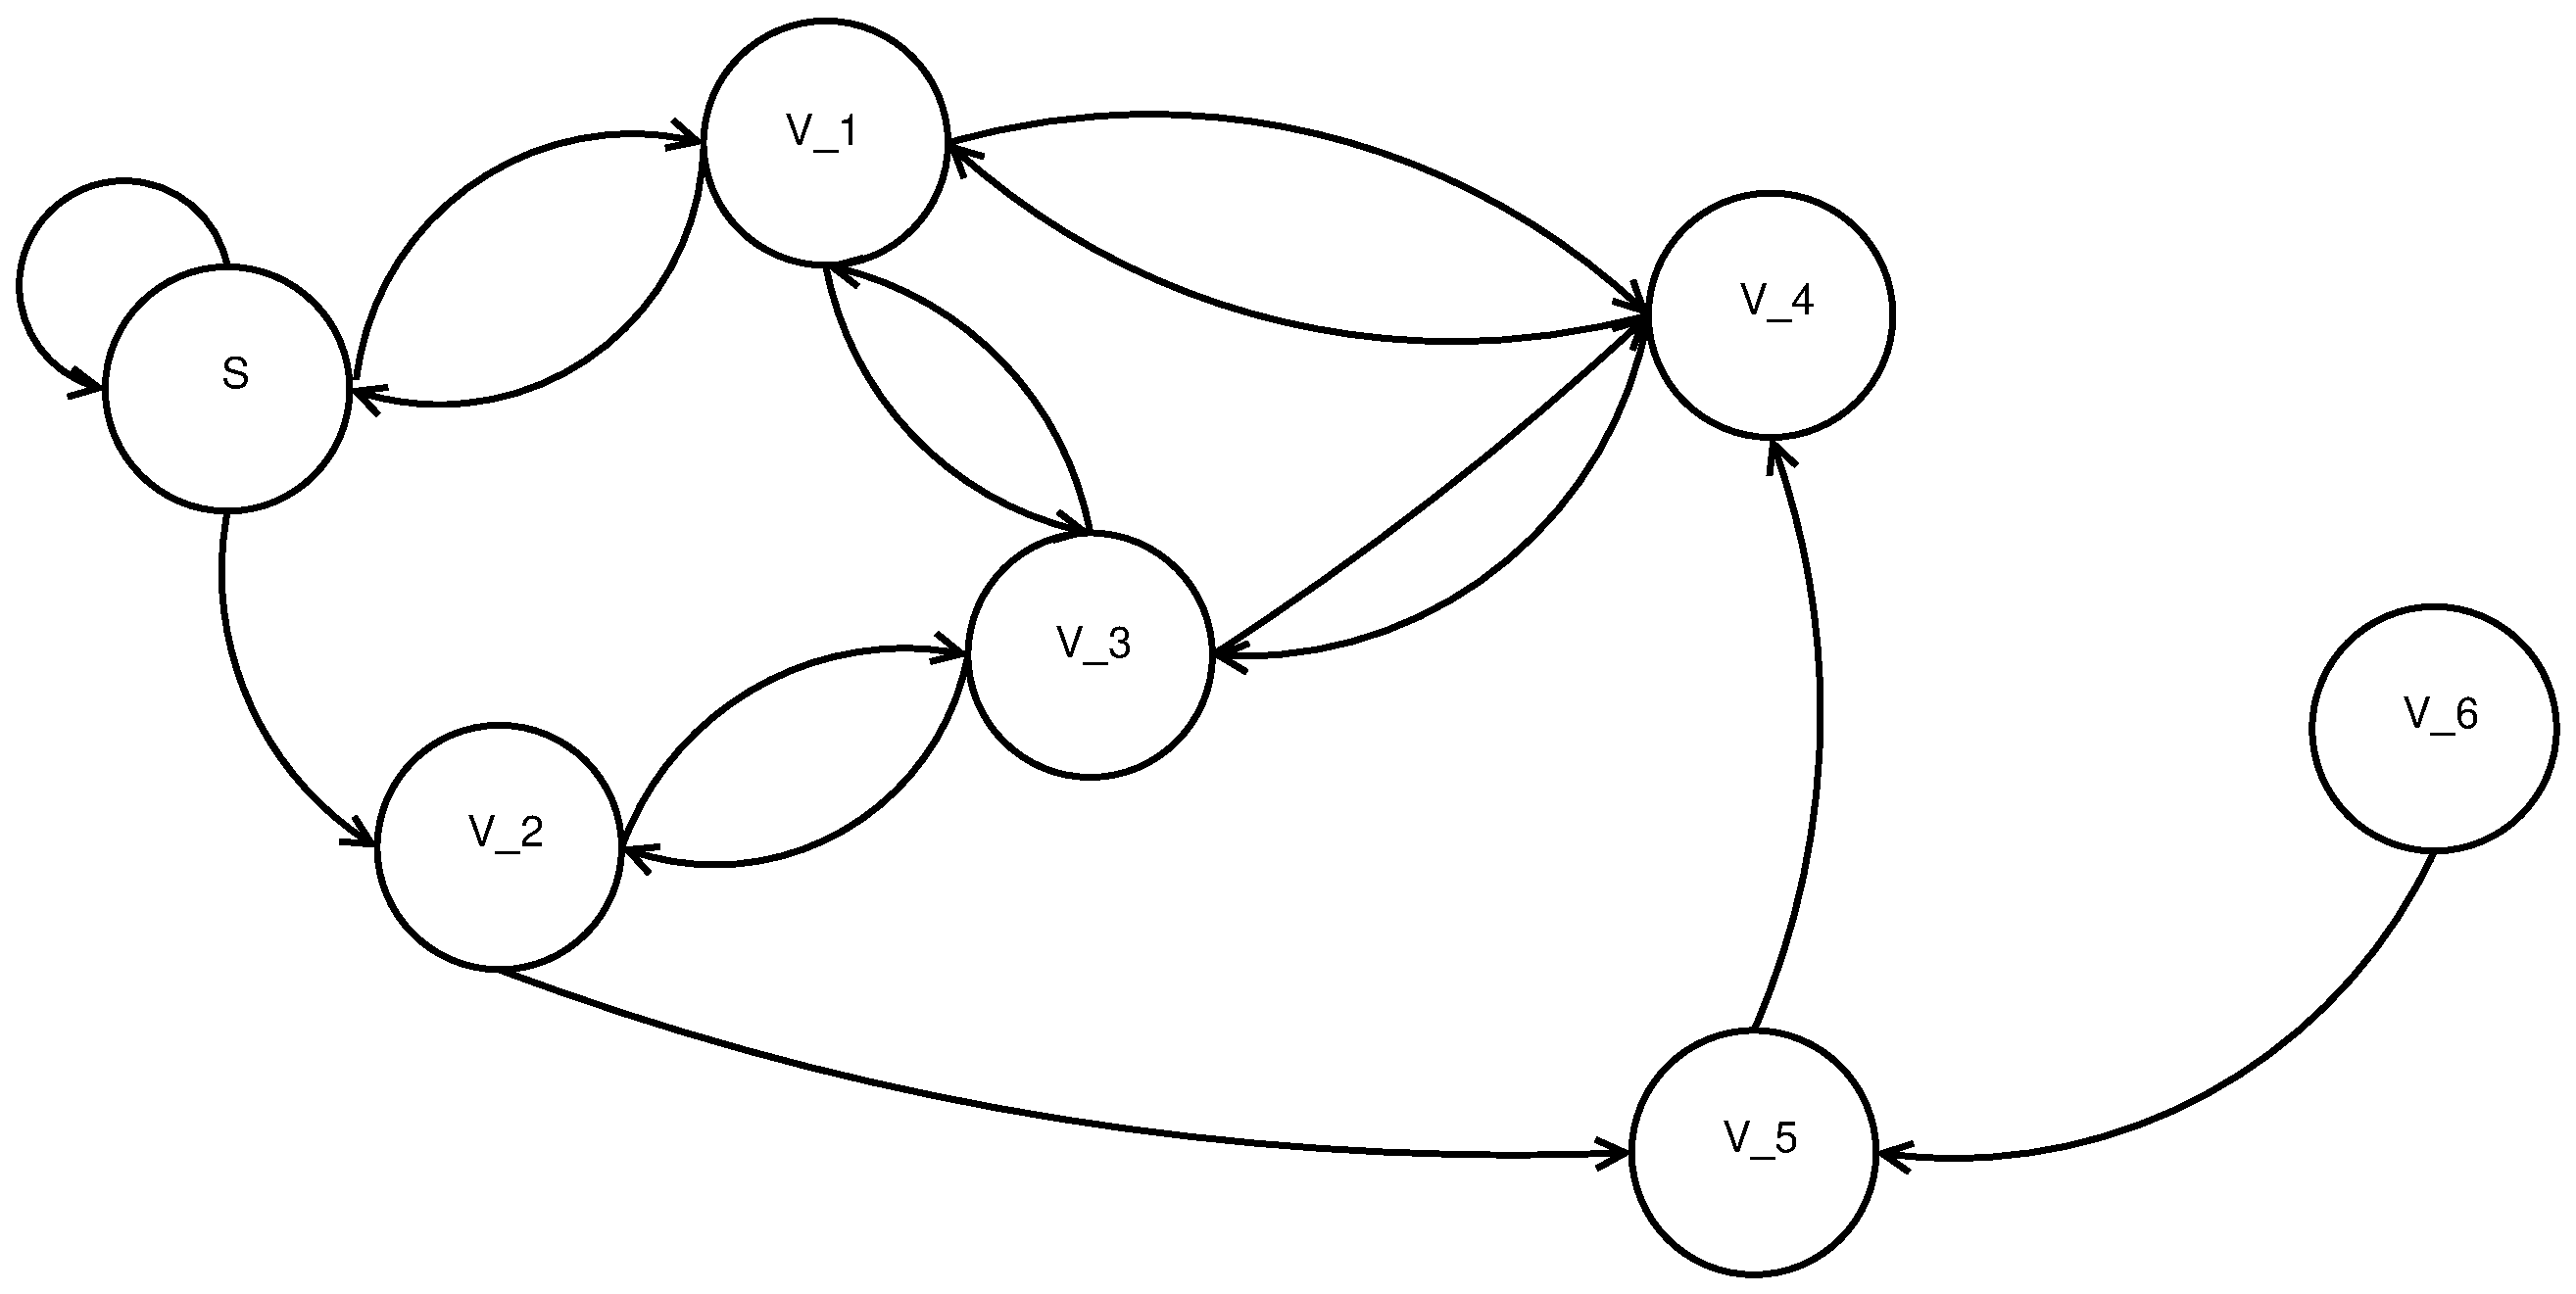
\includegraphics[width=0.5\linewidth]{15/Grafik/GerichteterGraph}
\caption{Gerichteter Graph}
\label{fig:GerichteterGraph}
\end{figure}

Planare Graphen können ohne Überkreuzung der Kanten in die Ebene eingebettet werden.

\section{Eulerische Polyederformel}
\begin{wrapfigure}{r}{0.25\linewidth}
	\centering
	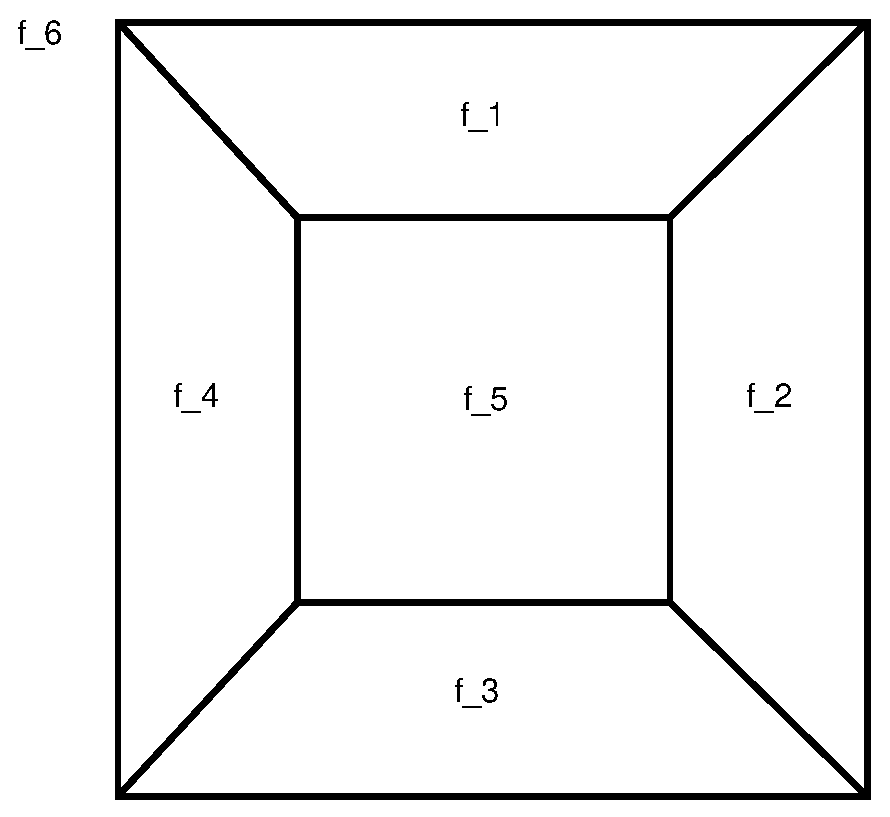
\includegraphics[width=\linewidth]{15/Grafik/Polyeder}
	\caption{Würfel}
	\label{fig:Polyeder}
	\vspace{-500pt}
\end{wrapfigure}

\[ |V| + |F| = |E| + 2 \]
\[ 8+6 = 12 + 2 \]
Es gilt: 
\[  2\cdot|E| \geq 3\cdot |F| \]
\begin{wrapfigure}{r}{0.25\linewidth}
	\vspace{-20pt}
	\centering
	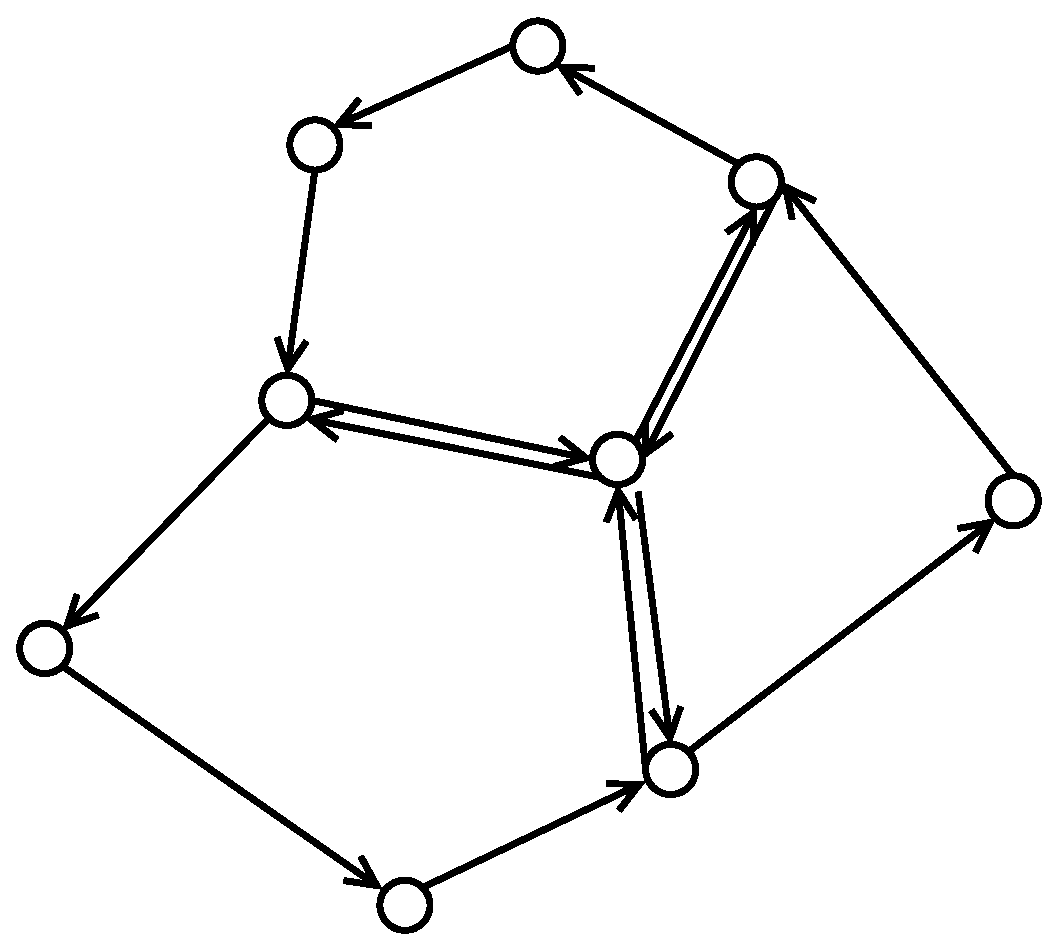
\includegraphics[width=\linewidth]{15/Grafik/Graph1}
	\caption{Placeholder}
	\label{fig:Graph1}
\end{wrapfigure}
\[ \text{\#gerichtete Kanten}= 2\cdot |E| = \sum_{i=1}^{|F|}\text{\#Kanten}(f_i)\footnote{Jedes $f_i$ hat mindestens 3 Kanten} \geq 3\cdot|F| \]
\[ |F| \leq \frac{2}{3}|E|,~~|V|+|F| = |E|+2\leq |V|+\frac{2}{3}|E| \Rightarrow \frac{1}{3}|E|+2 \leq |V|\]
\framebox{$\Rightarrow |E| \leq 3\cdot |V| -6$}
\begin{figure}[H]
\centering
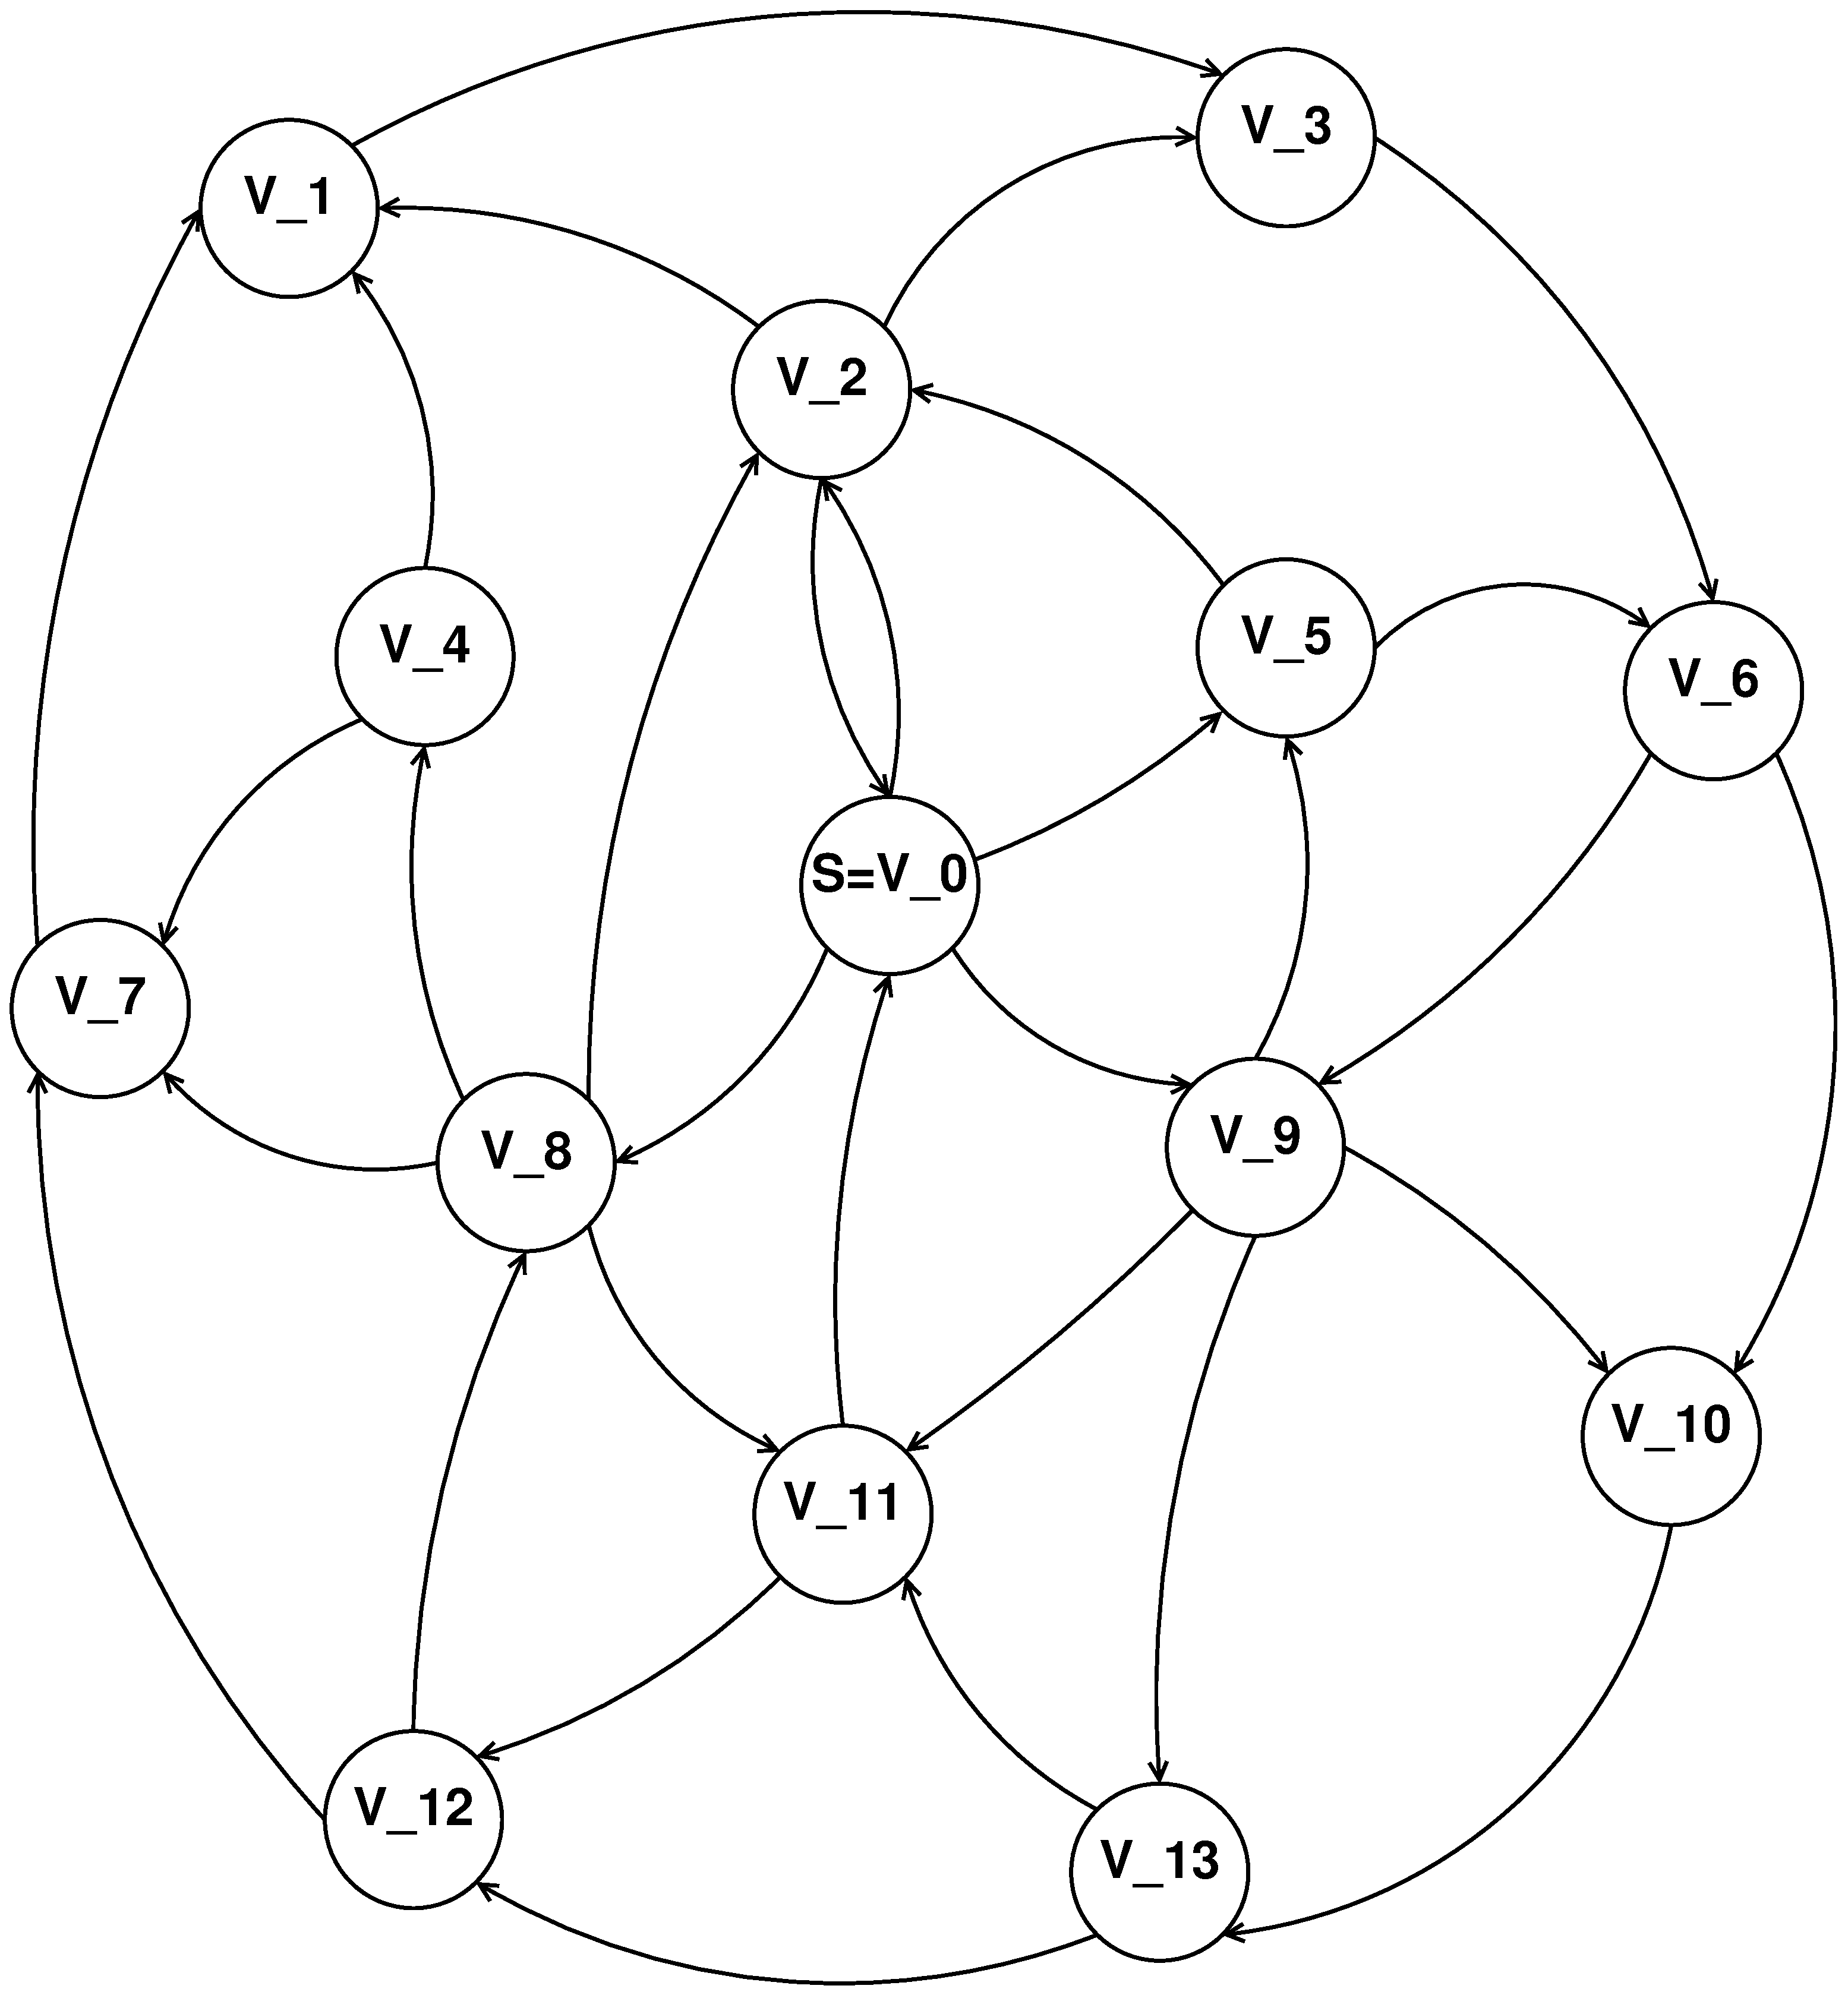
\includegraphics[width=0.5\linewidth]{15/Grafik/GerichteterGraph2}
\caption{Beispiel}
\label{fig:GerichteterGraph2}
\end{figure}

\section{Adjazenzmatrix}
\begin{tabular}{|c|cccccccccccccc|}
	\hline
	  &0&1&2&3&4&5&6&7&8&9&10&11&12&13 \\ \hline
	 0&1&0&1&0&0&1&0&0&1&1& 0& 0& 0& 0 \\
	 1&0&1&0&0&0&0&0&0&0&0& 0& 0& 0& 0 \\
	 2&1&1&1&1&0&0&0&0&0&0& 0& 0& 0& 0 \\
	 3&0&0&0&1&0&0&1&0&0&0& 0& 0& 0& 0 \\ \hline
	 4&0&1&0&0&1&0&0&1&0&0& 0& 0& 0& 0 \\ 
	 5&0&0&1&0&0&1&1&0&0&0& 0& 0& 0& 0 \\
	 6&0&0&0&0&0&0&1&0&0&1& 1& 0& 0& 0 \\
	 7&0&1&0&0&0&0&0&1&0&0& 0& 0& 0& 0 \\ \hline
	 8&0&0&1&0&1&0&0&1&1&0& 0& 0& 0& 0 \\
	 9&0&0&0&0&0&1&0&0&0&1& 1& 1& 0& 1 \\
	10&0&0&0&0&0&0&0&0&0&0& 1& 0& 0& 1 \\
	11&1&0&0&0&0&0&0&0&0&0& 0& 1& 1& 0 \\ \hline
	12&0&0&0&0&0&0&0&1&1&0& 0& 0& 1& 0 \\
	13&0&0&0&0&0&0&0&0&0&0& 0& 1& 1& 1 \\ \hline
	
\end{tabular}$= A$
\[ a\in B^{|V|\times |V|} \]
falls $G$ ungerichtet $\Rightarrow A = A^T$
\section{Adjazenzlisten Repräsentation}
\begin{figure}[H]
\centering
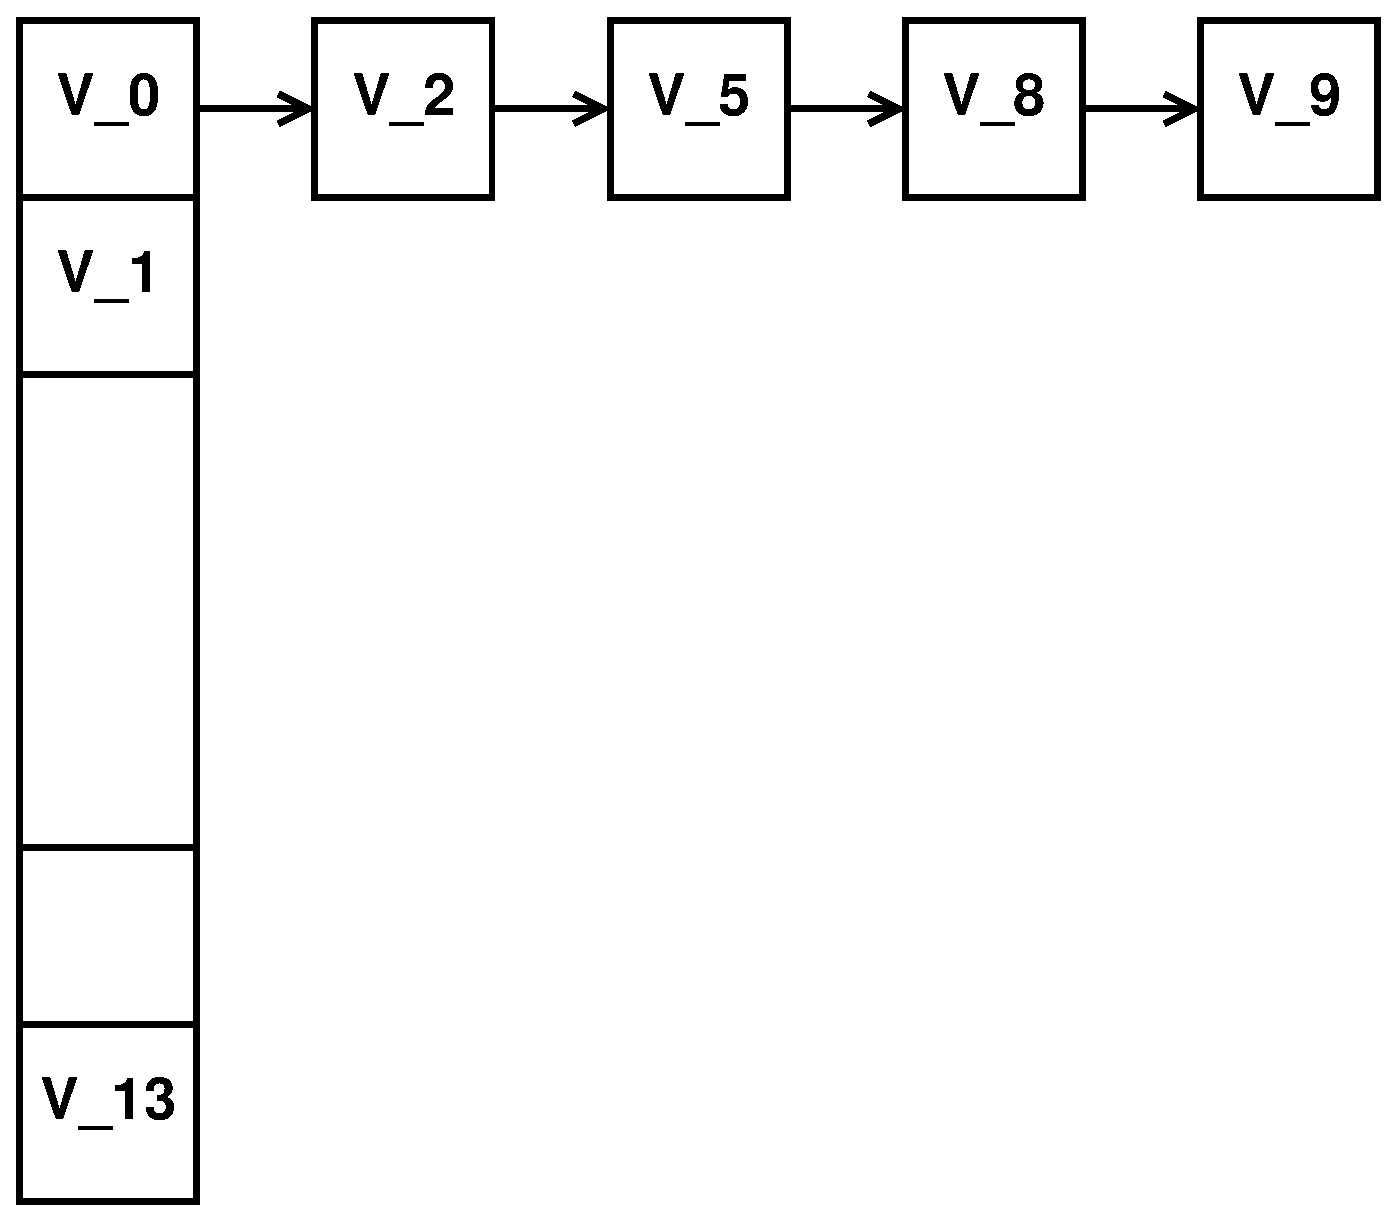
\includegraphics[width=0.4\linewidth]{15/Grafik/Liste}
\caption{Adjazenzliste}
\label{fig:Liste}
\end{figure}


\paragraph{Platzbedarf}
\[ \mathcal{O}(|V|+|E|)=\mathcal{O}\left( |V|+\sum_{i=0}^{|V|-1}\text{outdeg}(v_i) \right) \]
\begin{figure}[h]
\centering
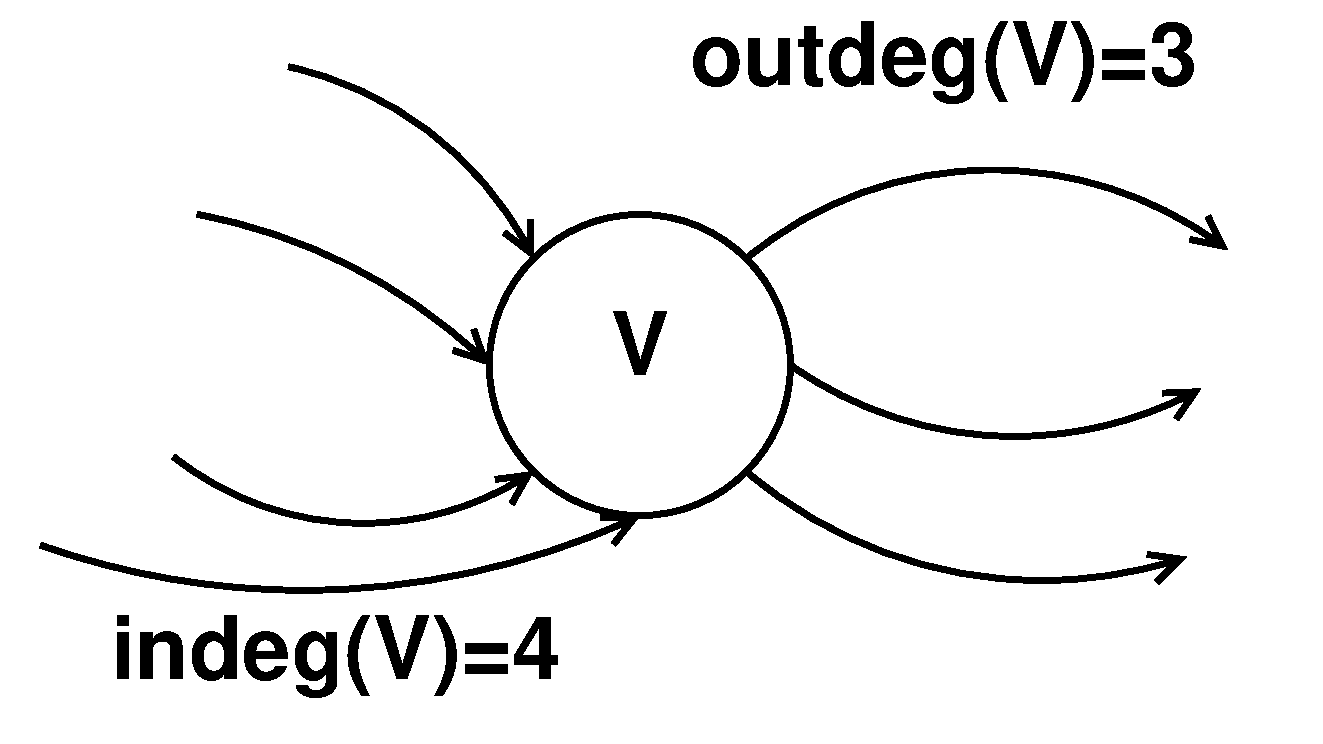
\includegraphics[width=0.3\linewidth]{15/Grafik/deg}
\caption{indeg und outdeg}
\label{fig:deg}
\end{figure}

\chapter{BFS (Breadth-First Search) Breitensuche}
\section{Pseudo-Code} %Ergänzung von Markus
\paragraph{Initialisierung}
\begin{lstlisting}[language=C, style = pseudo]
forall (v in V\{S}) {
  col[v]=white;    // Farbe  weiß = unbekannt, grau = bekannt, schwarz = vollkommen bekannt
  d[v] = infinity; // Distanz
  pi[v] = NULL;    // pi ist Vorgänger
}
col[s] = grey;     // s ist Startknoten
d[s] = 0;
pi[s] = NULL;
\end{lstlisting}
\begin{tabular}{ccc}
	Queue & vs & Stack \\
	Schlange &$~$& Stapel \\
	empty() &$~$ & '' \\
	push() &$~$ & '' \\
	pop() &$~$ &  \\
	FIFO &$~$ & FILO \\
	First-In-First-Out &$~$& First-In-First-Out 
\end{tabular}
\begin{wrapfigure}{r}{0.4\textwidth}
	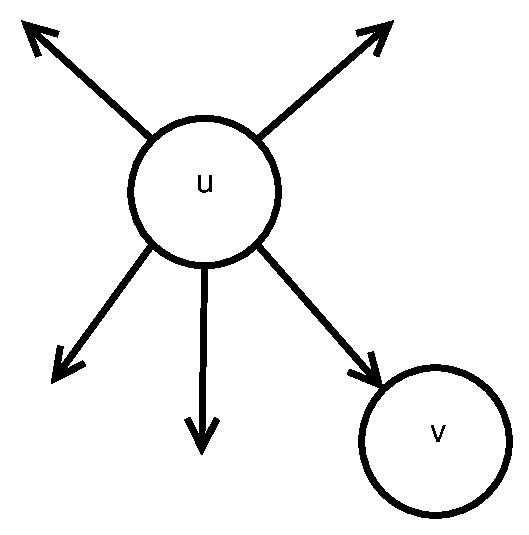
\includegraphics[width=\linewidth]{15/Grafik/CodeBild}
	\caption{Grafik zum Beispielcode}
	\label{fig:CodeBild}
\end{wrapfigure}
\begin{lstlisting}[style = pseudo]
Queue Q;
Q.push(s);
while(!Q.empty()) {
  u = Q.pop();
  forall( (u,v) in E) {
    if (col[v] == white) {
      col[v] == grey;
      d[v] = d[u]+1;
      pi[v] = u;
      Q.push(v);
    }
  }
  col[u] = black;
}
\end{lstlisting}

\section{Laufzeit} %Ergänzung von Markus, vorher \paragraph{Laufzeit}
\[ \mathcal{O}(|V|+|E|) \]
\paragraph{Begründung:}
Jeder von $s$ aus erreichbare Knoten wird nur einmal in die Queue aufgenommen und auch ihr entfernt. Für jeden Knoten muss nur einmal seine Adjazenzliste durchlaufen werden.
\[  \Rightarrow \mathcal{O}\left(|V|+\sum_{v \in V}\text{outdeg}(v) \right) \]

\clearpage